\documentclass[11pt]{beamer}
\usetheme{Warsaw}
\usepackage[utf8]{inputenc}
\usepackage{amsmath}
\usepackage{amsfonts}
\usepackage{amssymb}
\usepackage{amsfonts}
\usepackage{amssymb}
\usepackage{amsthm}
\usepackage{amsmath}
\usepackage{amsopn} 

\author{Rahul Jaiswal and Apoorve Kalot}
\title{Introduction to AI and ML}
\subtitle{Matrix Assignment}
\date{14/02/2019} 

\begin{document}

\begin{frame}
\titlepage
\end{frame}

\begin{frame}{Index}
\begin{enumerate}
\item Problem Statement
\item Steps to solve the problem
\item Theoretical Solution
\item Code
\item Figure
\end{enumerate}
\end{frame}

\begin{frame}{Problem Statement}
A straight line through the origin O meets the lines
\begin{equation}
(4 \ \ 3)x=10
\end{equation}
\begin{equation}
(8 \ \ 6)x+5=0
\end{equation}
at A and B respectively.Find the ratio in which O divides AB.
\end{frame}

\begin{frame}{Steps to solve the problem}
\begin{enumerate}
\item Pick a random point and determine the normal and direction vector of line AB passing through origin and this point
\item Determine the normal and direction vectors of given two lines
\item Determine the points of intersecion of this lines with line AB
\item Determine the ratio in which origin divides AB
\end{enumerate}
\end{frame}

\begin{frame}{Theoretical solution}
\begin{itemize}
\item \textbf{Picking random point B and Determining Dir-Vec AB }
The points are A = (0  0) and B = (0  10/3) 
 
 \[\left(\begin{array}{cc}
 A & B
 \end{array}\right)
 %
\begin{matrix}
=
\end{matrix}
\
%
\left(\begin{array}{cc}
0 & 0\\
0 & 10/3
\end{array}\right)
\]

The Direction Vector of AB is 
 
\[\left(\begin{array}{cc}
0 & 0\\
0 & 10/3
\end{array}\right)
\
%
\left(\begin{array}{cc}
-1\\
1
\end{array}\right)
%
\begin{matrix}
=
\end{matrix}
\
%
\left(\begin{array}{cc}
0\\
10/3

\end{array}\right)
\]

The normal Vector of AB is 
\[\left(\begin{array}{cc}
0 & 1\\
-1 & 0
\end{array}\right)
\
%
\left(\begin{array}{cc}
0\\
10/3
\end{array}\right)
%
\begin{matrix}
=
\end{matrix}
\
%
\left(\begin{array}{cc}
10/3\\
0

\end{array}\right)
\]

In the similar way Direction Vector and Normal Vector for Lines are 
\[\left(\begin{array}{cc}
3\\
-4
\end{array}\right)
\
%
\begin{matrix}
and
\end{matrix}
\
%
\left(\begin{array}{cc}
4\\ 
3
\end{array}\right)
\]

\end{itemize}
\end{frame}

\begin{frame}
\begin{itemize}
\item \textbf{Now we will find intersection points of line OB with given two lines}
Equation of line OB and given line are
\[\left(\begin{array}{cc}
1 & 1
\end{array}\right)
%
\left(\begin{array}{cc}
x\\
y
\end{array}\right)
\begin{matrix}
=
\end{matrix}
\
%
\begin{matrix}
0
\end{matrix}
\begin{matrix}
and
\end{matrix}
\
\left(\begin{array}{cc}
4\\
3
\end{array}\right)
\left(\begin{array}{cc}
x\\
y
\end{array}\right)
\begin{matrix}
=
\end{matrix}
\
%
\begin{matrix}
10
\end{matrix}
\]

This can be written as matrix equation
\[\left(\begin{array}{cc}
1 & 1\\
4 & 3
\end{array}\right)
\
%
\left(\begin{array}{cc}
x\\ 
y
\end{array}\right)
\begin{matrix}
=
\end{matrix}
\
%
\left(\begin{array}{cc}
0\\ 
10
\end{array}\right)
\]

So point of intersection 

\[\left(\begin{array}{cc}
x\\
y
\end{array}\right)
\
\begin{matrix}
=
\end{matrix}
\
\left(\begin{array}{cc}
-3 & 1\\ 
4 & -1
\end{array}\right)
\left(\begin{array}{cc}
0\\ 
10
\end{array}\right)
\]

So we got

\[\left(\begin{array}{cc}
x\\
y
\end{array}\right)
\
\begin{matrix}
=
\end{matrix}
\
%
\left(\begin{array}{cc}
10\\
-10
\end{array}\right)
\]
\end{itemize}
\end{frame}

\begin{frame}
\begin{itemize}
\item \textbf{Similarly we get point of intersection with second line as}
\[\left(\begin{array}{cc}
x'\\
y'
\end{array}\right)
\
%
\begin{matrix}
=
\end{matrix}
\
%
\left(\begin{array}{cc}
-5/2\\
5/2
\end{array}\right)
\]
Distance from Origin to this two points are 14.142 and 3.5355
So Ratio is 4.0
\end{itemize}
\end{frame}

\begin{frame}{Code}
\href{https://github.com/rahul-1510/Introduction-to-AI-ML}{\beamergotobutton{Link}}
\end{frame}

\begin{frame}{Figure}
\frametitle{Solution Figure-}
		\begin{figure}
    		\centering
    		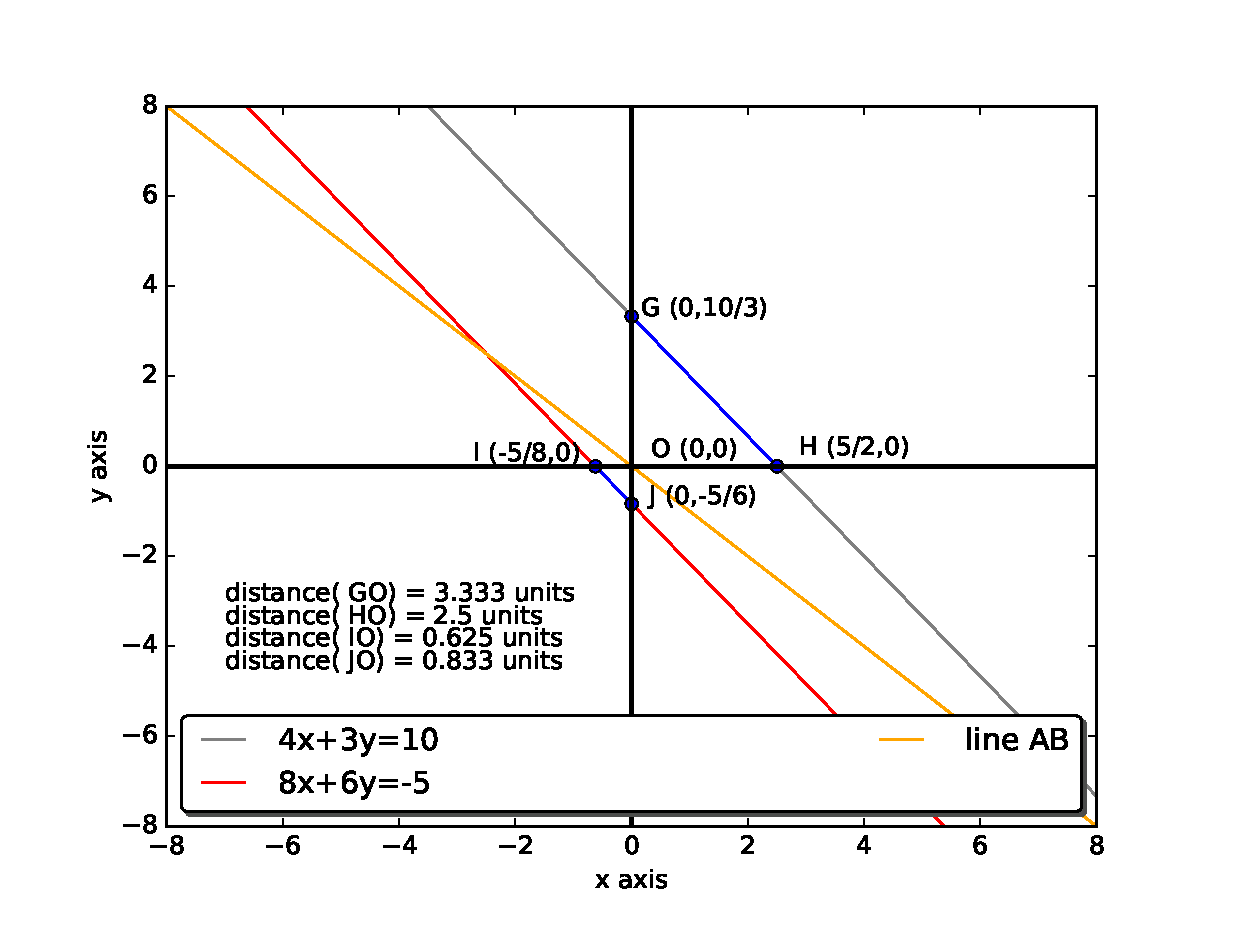
\includegraphics[width = 0.9\textwidth]{./assign1op.eps}
  		\end{figure}
\end{frame}

\end{document}

\grid
\grid
